
\chapter{在光学腔中利用相干光场制备原子系综的纠缠态}\label{chapter4}
\vbox{}\vbox{}
原子系综的纠缠在量子信息处理与量子精密测量中有着重要的应用,其是实现远距离量子通信、构建高效量子存储器的基础。本文提出了一种简单但易于实验实现的理论方案用以制备原子系综间的纠缠,即通过向光学腔中注入相干(经典)光场,以相干光场为驱动力,同时利用腔模的量子输运效应实现两个原子系综之间的高斯纠缠。我们发现本方案所产生的纠缠根植于量子非破坏性测量相互作用,而这一类型相互作用在连续变量计算中有也有着很重要的应用。

\vbox{}
\section{引言}
\vbox{}
量子纠缠是量子力学中许多问题的核心\cite{bouwmeester2000physics,horodecki2009quantum,knill2005quantum},近年来正在引起越来越多的关注。在若干量子信息\cite{bennett1993teleporting,bennett1992communication,beige2001secure}处理问题中都需要用到纠缠,例如在量子远程传送\cite{pirandola2015advances,herbst2017quantum}和量子通信\cite{gisin2007quantum,ursin2007entanglement}以及在某些量子加密协议中\cite{broadbent2019uncloneable,yang2018mutual}都需要用到它。它在量子计算\cite{maezawa2018toward,grover1996fast}中也发挥着重要作用,使得量子计算机可以在诸如素数因子分解或搜索\cite{nielsen2002quantum,ekert1996quantum,vandersypen2001experimental}等几个问题上超越经典计算机。此外,在研究量子力学中的某些非经典现象时,量子纠缠的产生也成为当今量子调控实现的目标。

原子系综作为量子纠缠的载体,因为其具备易于实现与弱光场的相互作用以及抵御体系退相干等诸多优点而正引起研究者的极大兴趣。迄今为止,已有多种方案被提出用于制备原子系综的纠缠态。其中一种方法是光场记忆法\cite{lukin2000entanglement},即通过将纠缠光场分别存储到两个原子系综用以建立原子间的纠缠;另外一种方法是投影测量法\cite{duan2000quantum},即首先建立光与原子间的纠缠,而后对出射光场做投影测量即可实现体系的纠缠交换,从而实现原子与原子间的纠缠。对于光场记忆法,显然原子系综的纠缠度受制于光场的纠缠度以及光记忆的保真度;而对于投影测量法体系的纠缠度受制于探测器的探测效率。本文提出了一种不同此两种的新方法,即将原子系综放置于光学腔中,通过相干光场驱动,利用腔模的“量子公共汽车”效应建立起原子之间的非经典关联。与之前的方法相比,我们的方案即不需要非经典的量子资源,也不需要高效的量子态探测技术,故可极大地简化实验实施过程,提高纠缠产生的效率。

我们所研究的量子系统是由大量原子自旋组成的原子系综,对于由N个自旋1/2粒子的系统,我们可定义可观察量的集体角动量算符
\begin{align}\label{eq551}
	{J_l} = \frac{1}{2}\sum\limits_{k = 1}^N {\sigma _l^{(k)}} ,
\end{align}
其中$l=x,y,z$,$\sigma_l^{k}$是Pauli矩阵。三个正交方向上的自旋分量之间满足对易关系$[J_x,J_y]=i\hbar J_z$,这里的${J_x} = ({J_ + } + {J_ - })/2$和${J_y} = ({J_ + } - {J_ - })/2i$,其中$J_+(J_-)$表示原子的升(降)算符。如果系综里的所有原子朝着$x$方向极化,则我们可利用Holstein-Primakoff近似\cite{zhang1998even}将轨道角动量振子化,即可定义新的原子量子变量${X_a} = {J_y}/\sqrt {{J_x}} $,${P_a} = {J_z}/\sqrt {{J_x}} $,满足 $[ X_a, P_a] = i$。对于CSS,有$\braket{ X_a}=\braket{ P_a} = 0$和归一化方差${(\Delta {X_a})^2} = {(\Delta { P_a})^2} = 1/2$。
于是,原子系综间的纠缠问题转化为振子间的连续变量纠缠问题。本文的结构主要如下:在第二部分我们首先并给出了两个原子系综之间产生纠缠的详细过程,并对产生的纠缠进行了判据;第三部分我们简要分析了噪声对纠缠的影响;第四部分是结论的和分析。
\begin{figure}[htbp]
	\centering
	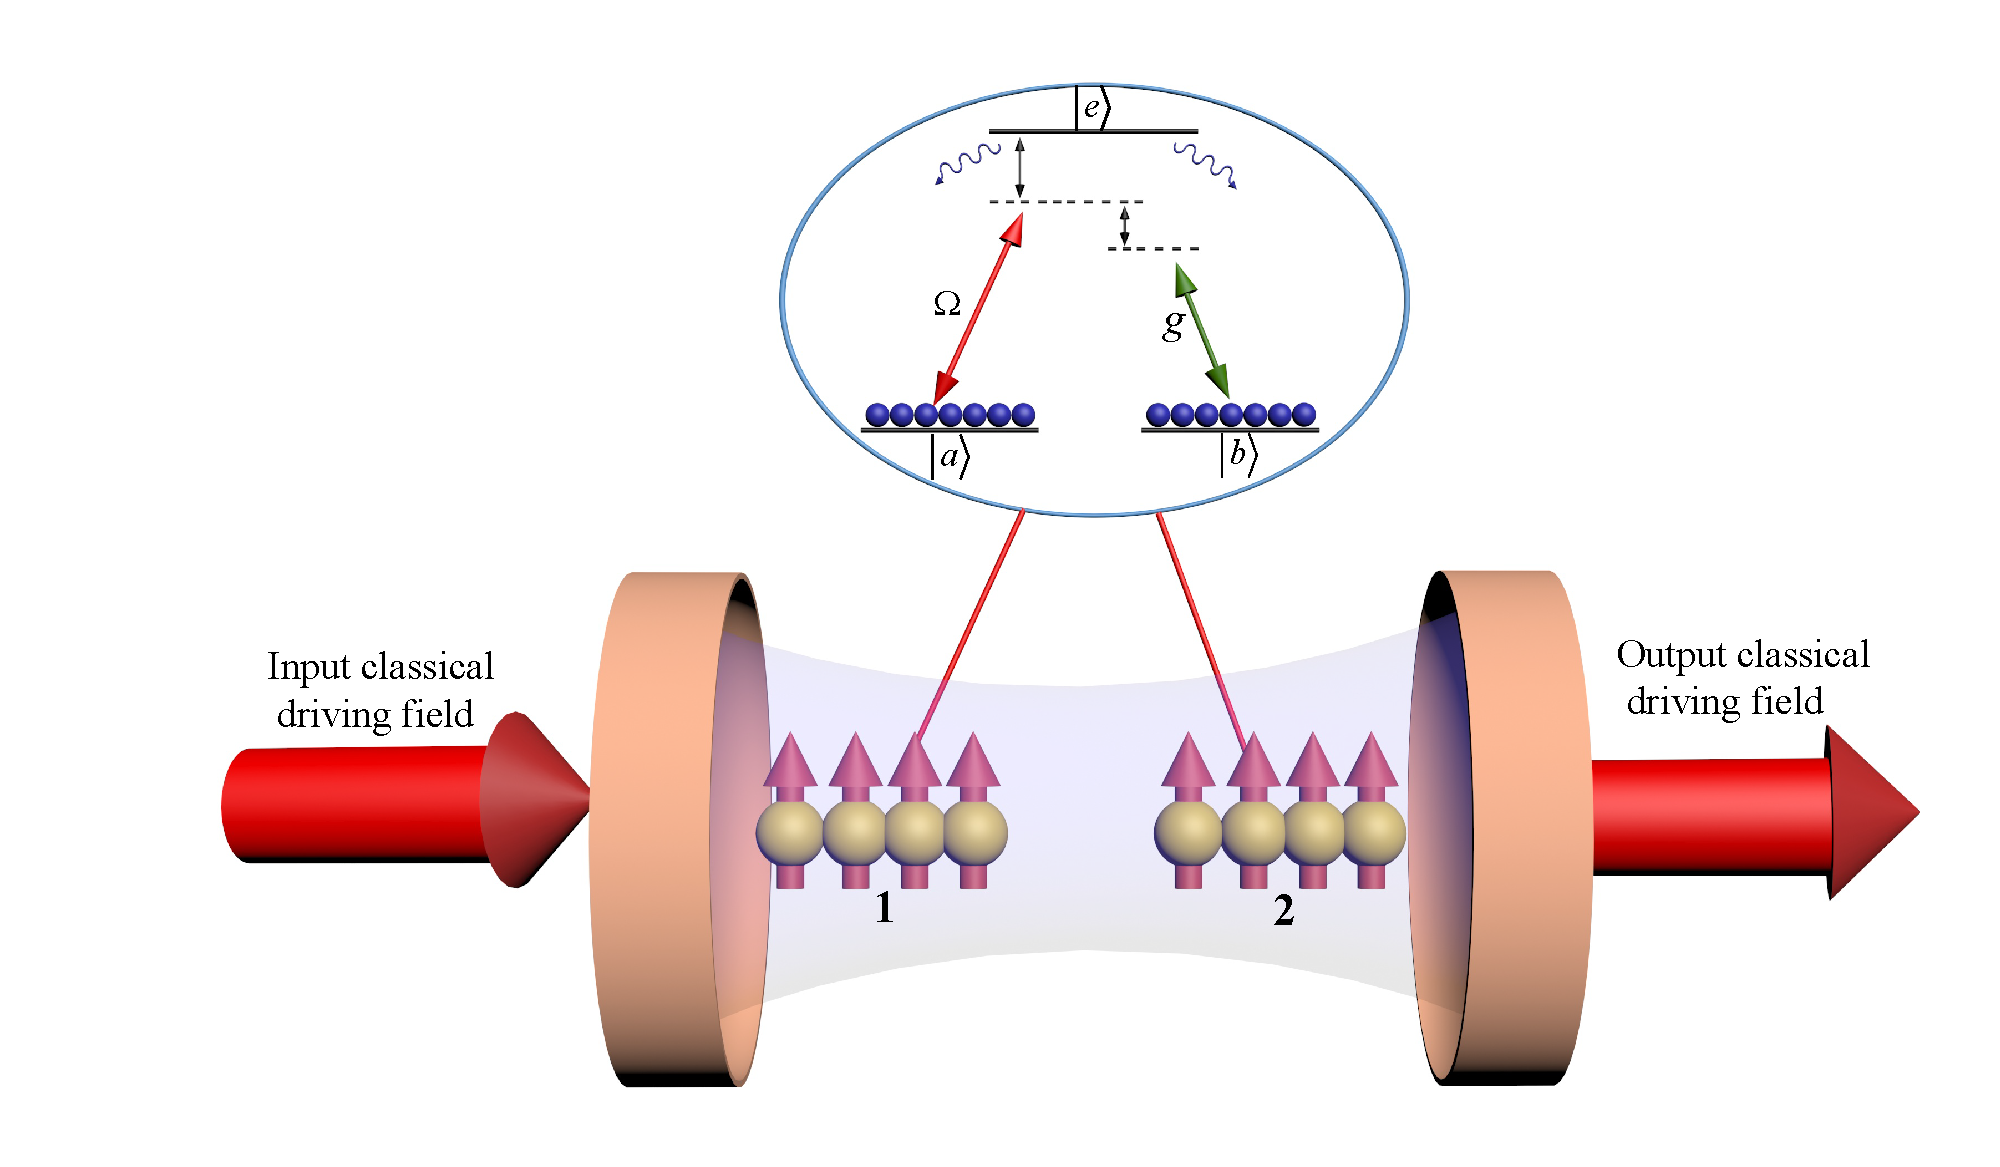
\includegraphics[scale=0.35]{Img/Fig_551.pdf}
	\bicaption{$\Lambda$型的原子系综和腔场的耦合示意图。一束激光与两原子系综的基态$\ket{a}$和激发态$\ket{e}$实现非共振耦合,而基态$\ket{b}$和激发态$\ket{e}$与处于真空态的腔模相耦合,绝热消除原子的激发态与腔模后即可得到原子的等效演化,该演化正是原子间纠缠产生的根源。}	
	{Schematic diagram of the $\Lambda$-type atomic ensemble coupling with cavity field. A laser beam couples off-resonantly with two atomic ensembles by the ground state $\ket{a}$ and the excited state $\ket{e}$, while the ground state $\ket{b}$ and the excited state $\ket{e}$ are coupled with the cavity mode in the vacuum state. By adiabatic elimination of the atom excited state and the cavity mode, one obtains and effective evolution of atoms, which is the source of entanglement between atoms.}
	\label{figure51}
\end{figure}

\vbox{}
\section{纠缠态的产生}
\vbox{}
考虑有两个完全相同的$\Lambda$型的三能级原子系综置于单模腔场中并与腔场相互作用的模型,其原子数分别为$N_1$和$N_2$,能级结构示意图如图\ref{figure51}所示。原子有两个稳定的基态$\ket{a}$、$\ket{b}$和激发态$\ket{e}$,两个基态之间的能级差是$\omega_{ab}$(这里我们取$\hbar=1$),基态$\ket{a}$和激发态$\ket{e}$之间的能级差是$\omega_{ae}$。基态$\ket{a}$和激发态$\ket{e}$之间通过一个频率为$\omega$经典驱动场相耦合,其共振拉比频率为$\Omega$,与基态$\ket{b}$之间的耦合则通过与腔模$c$的相互作用来完成。

对于这两个三能级原子系综与单模腔场相互作用的系统,我们可以很容易的写出系统的哈密顿量为
\begin{align}\label{eq552}
	\begin{split}
		\hat H   =& \omega_0\hat c^\dag \hat c+\sum_{i}^{2}[\sum_k \omega_{ae}\ket{e}_k\bra{e}
		+ H_I]_i \\
		&H_I= \sum_k (\frac{\Omega}{2}e^{-i\omega t}\ket{e}_k\bra{a}
		+g\hat c\ket{e}_k\bra{b}+h.c.),
	\end{split}
\end{align}
其中$\hat c$和$\hat c^\dagger$表示光场的湮灭和产生算符,$\omega_0$是相应腔模的频率,$g$是原子与腔场的耦合常数,下标1和2分别表示1和2号原子系综的算符,$\sum_i^2$表示对两个原子系综的哈密顿量求和。

接下来我们令$\hat \sigma_{\mu\nu}=\sum_k{\ket{\mu}_k\bra{\nu}}$(其中$\mu,\nu\in {1,2,3}$)对公式(\ref{eq552})中的哈密顿量进行化简,则有
\begin{align}\label{eq553}
	\begin{split}
		\hat H   = \omega_0\hat c^\dag \hat c + \omega_{ae}\sigma_{ee}
		+(\frac{\Omega}{2}e^{-i\omega t}\sigma_{ea}+g\hat c\sigma_{eb}+h.c.),
	\end{split}
\end{align}
其中我们定义了算符
\begin{align}	\label{eq554}
	\begin{split}
		\omega_{ae}\sigma_{ee}                   &= (\omega_{ae}\sigma_{ee})_1
		+(\omega_{ae}\sigma_{ee})_2,\\
		\frac{\Omega}{2}e^{-i\omega t}\sigma_{ea}&= (\frac{\Omega}{2}e^{-i\omega t}\sigma_{ea})_1
		+(\frac{\Omega}{2}e^{-i\omega t}\sigma_{ea})_2,\\
		g\hat c\sigma_{eb}                       &= (g\hat c\sigma_{eb})_1
		+(g\hat c\sigma_{eb})_2,
	\end{split}
\end{align}
通过上式我们可以看到,两个小原子系统的总哈密顿量可以写成一个大原子系综的哈密顿量。我们也可以很容易的写出$J_l=J_{l1}+J_{l2}$,其中$l=x,y,z$。

接下来我们进入一个转动坐标系,这一转动由哈密量$\hat H_0^1= \omega_0\hat c^\dag \hat c + \omega_{ae}\sigma_{ee}$来统治,对公式\ref{eq553}的哈密顿量进行旋转后,得到
\begin{align}\label{eq555}
	\begin{split}
		\hat{ H}_{eff}^1 &= {e^{i{{\hat H}_0}t/\hbar }}\hat H{e^{ - i{{\hat H}_0}t/\hbar }} 
		- {{\hat H}_0}\\
		&= \Delta {{\hat \sigma }_{33}} + \frac{\Omega }{2}{{\hat \sigma }_{31} }
		+ g\hat \varepsilon {{\hat \sigma }_{32}} 
		+ \frac{{{\Omega ^*}}}{2}{{\hat \sigma }_{13}}
		+ g{{\hat \sigma }_{23}}{{\hat \varepsilon }^\dag },
	\end{split}
\end{align}
式中我们定义了一个新算符$\hat \varepsilon  = \hat c{e^{i\delta t}}$。根据哈密顿量,我们可以计算出光和原子的海森堡方程,得到如下的Maxwell-Bloch方程
\begin{align}\label{eq556}
	\begin{split}
		{\dot{\hat{ \sigma}} _{11}}  & =  i\frac{\Omega }{2}{\hat \sigma _{31}} 
		- i\frac{{{\Omega ^*}}}{2}{\hat \sigma _{13}},\\
		{\dot {\hat{ \sigma}} _{22}} & =  ig\hat \varepsilon {\hat \sigma _{32}} 
		- i{g^*}{\hat \sigma _{23}}{\hat \varepsilon ^\dag },\\
		{\dot {\hat{ \sigma}} _{12}} & =  i\frac{\Omega }{2}{\hat \sigma _{32}} 
		- i{g^*}{\hat \sigma _{13}}{\hat \varepsilon ^\dag },\\
		{\dot {\hat{ \sigma}} _{13}} & =- i\Delta {\hat \sigma _{13}} 
		- i\frac{\Omega }{2}\left( {{{\hat \sigma }_{11}} - {{\hat \sigma }_{33}}} \right) - ig\hat \varepsilon {\hat \sigma _{12}},\\
		{\dot {\hat{ \sigma}} _{23}} & =- i\Delta {\hat \sigma _{23}}-i\frac{\Omega }{2}{\hat \sigma _{21}}
		- ig\hat \varepsilon \left( {{{\hat \sigma }_{22}} 
			- {{\hat \sigma }_{33}}} \right),\\
		{\dot {\hat{ \sigma}} _{33}} & =  i\frac{{{\Omega ^{\rm{*}}}}}{2}{\hat \sigma _{13}}
		- i\frac{\Omega }{2}{\hat \sigma _{31}} 
		+ i{g^{\rm{*}}}{\hat \sigma _{23}}{\hat \varepsilon ^ + } 
		- ig\hat \varepsilon {\hat \sigma _{32}},\\
		\dot {\hat{ \varepsilon}}    & =- i{g^*}{\hat \sigma _{23}} + i\delta \hat \varepsilon , 
	\end{split}
\end{align}
接下来,为了方便计算,我们做如下的假设:1.假设经典驱动场足够的弱。2.假设失谐量$\Delta\gg 1$。通过这样的假设,可以认为布居在激发态的原子数非常少,因此可以绝热消除掉激发态(${\sigma _{33}} \simeq 0$)。大失谐还可以将$\sigma_{13}$和$\sigma_{23}$快速驱动到稳态,于是有${\hat \sigma _{13}} \simeq  - \left( {\Omega {{\hat \sigma }_{11}}/2 + g\hat \varepsilon {{\hat \sigma }_{12}}} \right)/\Delta $,${\hat \sigma _{23}} \simeq  - \left( {\Omega {{\hat \sigma }_{21}}/2 + g\hat \varepsilon {{\hat \sigma }_{22}}} \right)/\Delta $ 。我们进一步假设双光子失谐量足够大$\delta\gg 1$,使得在相互作用期间腔中没有产生显着的光子激发,这使得能够绝热地消除腔场,导致$\hat \varepsilon  =  - {g^*}\Omega {\hat \sigma _{21}}/2\Delta \delta $。基于这些假设,原子的基态方程可以写为
\begin{align}
	{\dot{ \hat{ \sigma}} _{12}} =  - i{\kappa _0}{\hat S_z}{{ \hat{ \sigma}} _{12}}
	- i{\chi _0}{{ \hat{ \sigma}} _{12}},{\dot { \hat{ \sigma}} _{11}} = {\dot { \hat{ \sigma}} _{22}} = 0,\label{eq557}
\end{align}
其中定义了$\kappa_0=|\Omega|^2{|g|^2}/4{\delta\Delta^2}$ 和 $\chi_0 ={|\Omega|^2}/{4\Delta}$。在伪角动量运算符的表述中,公式(\ref{eq557})可以写为
\begin{align}\label{eq558}
	\begin{split}
		{{\dot {\hat J}}_x} &=  {\kappa _0}\left( {{{\hat J}_y}{{\hat J}_z} 
			+ {{\hat J}_z}{{\hat J}_y}} +{{\hat J}_y}\right) 
		+ {\chi _0}{{\hat J}_y},\\
		{{\dot {\hat J}}_y} &=- {\kappa _0}\left( {{{\hat J}_x}{{\hat J}_z} 
			+ {{\hat J}_z}{{\hat J}_x}} +{{\hat J}_x}\right) 
		- {\chi _0}{{\hat J}_x},\\
		{{\dot {\hat J}}_z} &= 0,
	\end{split}
\end{align}
从上面的这组方程,可以推断原子的动力学是由下式的有效哈密顿量产生的
\begin{align}
	\hat H_{eff}^2=-\chi_0\hat S_z-\kappa_0(\hat S_z+\hat S_z^2),
	\label{eq559}
\end{align}
从哈密顿量的形式我们知道这是一个OAT型的哈密顿量\cite{PRA1993Kitagawa}。(\ref{eq559})式的第一项出现源于基态的AC-Stark平移,而其余项源于双光子非共振拉曼跃迁。通过取参数$\chi_0=-\kappa_0$,公式(\ref{eq559})中的有效哈密顿量将变成一个纯粹的OAT哈密顿量,即$\hat H_{eff}=\chi_0 S_z^2$。

将系统总的自旋用两个小系综的自旋之和来表示,于是我们可以将系统的哈密顿量重新写为如下的形式,
\begin{align}\label{eq5510}
	\begin{split}
		\hat H_{eff}^3& = {\chi _0}J_z^2\\
		&= {\chi _0}{({J_{z1}} + {J_{z2}})^2}\\
		&= {\chi _0}(J_{z1}^2 + J_{z2}^2 + 2{J_{z1}}{J_{z2}}),
	\end{split}
\end{align}
然后我们进入$\hat H_0^2 = J_{z1}^2 + J_{z2}^2$的转动坐标系,可以得到在新的相互作用绘景下有效哈密顿量
\begin{align}\label{eq5511}
	\begin{split}
		\hat{H}_{eff}=\chi\hat{P}_1\hat{P}_2,
	\end{split}
\end{align}
其中我们定义了$\chi=2\chi_0 \sqrt{J_{x1}J_{x2}}$。我们也定义了原子系综的动量位置算符$\left( {{{\hat X}_1},{{\hat P}_1}} \right)$和$\left( {{{\hat X}_2},{{\hat P}_2}} \right)$,其满足对易关系$\left[ {{{\hat X}_1},{{\hat P}_1}} \right] = \left[ {{{\hat X}_2},{{\hat P}_2}} \right] = i$,且有$\left\langle {{{\hat X}_1}} \right\rangle  = \left\langle {{{\hat X}_2}} \right\rangle  = \left\langle {{{\hat P}_1}} \right\rangle  = \left\langle {{{\hat P}_2}} \right\rangle  = 0$,$\left\langle {\hat X_1^2} \right\rangle  = \left\langle {\hat X_2^2} \right\rangle  = \left\langle {\hat P_1^2} \right\rangle  = \left\langle {\hat P_2^2} \right\rangle  = \frac{1}{2}$。接下来我们将证明在这个哈密顿量的作用下,两个原子系综之间存在着量子纠缠。

我们首先可以利用公式(\ref{eq5511})中给出的哈密顿量,计算出原子算符随时间的演化方程
\begin{align}\label{eq5512}
	{{\dot {\hat{ X}}}_1} = \chi {{\hat P}_2},
	{{\dot {\hat{ P}}}_1} = 0 ,
	{{\dot {\hat{ X}}}_2} = \chi {{\hat P}_1},
	{{\dot {\hat{ P}}}_2} = 0,
\end{align}
通过求解方程(\ref{eq5512}),我们得到
\begin{align}\label{eq5513}
	\left( {\begin{array}{*{20}{c}}
			{\hat X_1^{out}}\\
			{\hat P_1^{out}}\\
			{\hat X_2^{out}}\\
			{\hat P_2^{out}}
	\end{array}} \right) = \left( {\begin{array}{*{20}{c}}
			1   & 0     & 0   & \kappa\\
			0   & 1     & 0   & 0     \\
			0   &\kappa & 1   & 0     \\
			0   & 0     & 0   & 1
	\end{array}} \right)\left( {\begin{array}{*{20}{c}}
			{\hat X_1^{in}}\\
			{\hat P_1^{in}}\\
			{\hat X_2^{in}}\\
			{\hat P_2^{in}}
	\end{array}} \right)
\end{align}

其中$\kappa=\chi t$,“in”表示最初系统演化之前的量子态,“out”表示系统演化之后输出的量子态。

很显然,我们这里原子系综的量子态是高斯态,因为初始输入态是真空态,而相互作用的哈密顿量是正则算符平方,故相互作用过程不改变体系量子态的高斯特性\cite{simon2000peres},于是我们可以很方便的用Wigner函数来表示体系的量子态,即可得到
\begin{align}\label{eq5514}
	W(\xi)=\frac{1}{(2\pi)\sqrt{det V^{(2)}}}exp^{{-\frac12\xi[V^{(2)}]^{-1}\xi^T}},
\end{align}
这里$\xi = [{X_1},{P_1},{X_2},{P_2}]$是正则矢量算符,V是关联矩阵,关联矩阵的矩阵元计算方法如下所示\cite{braunstein2005quantum}
\begin{align}\label{eq5515}
	V_{ij}=\braket{(\hat{\xi}_i\hat{\xi}_j+\hat{\xi}_j\hat{\xi}_i)/2},
\end{align}
对于方程(\ref{eq5514})中的高斯态,Wigner函数完全由二阶关联矩阵确定。对于经典4维相空间上的经典概率分布,每个物理相关矩阵是正的、实数和对称的。与之对应的,任何实的、对称的正矩阵都表示可能的物理关联矩阵。除了正的、实数和对称的之外,描述量子相空间的Wigner相关矩阵(任意态)也必须满足如下的关系
\begin{align}\label{eq5516}
	[\hat{\xi}_k,\hat{\xi}_l]=\frac{i}{2}\Lambda_{k,l},k,l=1,2,3,4
\end{align}
对于4×4矩阵$\Lambda$,其具有2×2矩阵J作为每个正交对的对角项
\begin{align}\label{eq5517}
	\Lambda=\left( {\begin{array}{*{20}{cc}}
			J  & 0\\
			0  & J
	\end{array}} \right)
	,J=\left( {\begin{array}{*{20}{cc}}
			0  & 1\\
			-1 & 0
	\end{array}} \right).
\end{align}

现在让我们考虑任意双模态。根据公式(\ref{eq5515})中的双模关联矩阵$V^(2)$的定义,我们可以以分块的形式写出任意双模态的关联矩阵
\begin{align}\label{eq5518}
	V=\left( {\begin{array}{*{20}{cc}}
			A  & C\\
			C^T& B
	\end{array}} \right)
\end{align}
其中A,B和C是实的2×2的矩阵。Simon的Peres-Horodecki判据如下
\begin{align}\label{eq5519}
	\begin{split}
		F=\det{A}\det{B}+(\frac1{16}-|\det{C}|)^2&-Tr(AJCJBJC^TJ)\\
		&\ge G=\frac1{16}(\det{A}+\det{B}),
	\end{split}
\end{align}
其中J是公式(\ref{eq5517})中的2×2矩阵。任意的可分离的两高斯模满足不等式$F\ge G$,它代表了可分离性的必要条件,因此它的违反是不可分离性的充分条件。

利用前面公式(\ref{eq5515})给出的表达式,我们可以计算两原子系综与光场相互作用系统的关联矩阵,于是有
\begin{align}\label{eq5520}
	{V_{ij}} =\frac14 \left( 
	{
		\begin{array}{*{20}{c}}
			1+\kappa^2 &    0   &    0       & \kappa \\
			0      &    1   & \kappa     &    0   \\
			0      & \kappa & 1+\kappa^2 &    0   \\
			\kappa   &    0   &    0       &    1
		\end{array}
	} 
	\right),
\end{align}
接下来我们可以将$V_{ij}$方块化,得到
\begin{align}\label{eq5521}
	A=\left(
	{
		\begin{array}{*{20}{cc}}
			1+\kappa^2  & 0\\
			0        & 1
		\end{array}
	} 
	\right),
	B=\left(
	{
		\begin{array}{*{20}{cc}}
			1+\kappa^2  & 0\\
			0        & 1
		\end{array}
	} 
	\right),
	C=C^T=\left(
	{
		\begin{array}{*{20}{cc}}
			0       & \kappa\\
			\kappa     &   0 
		\end{array}
	} 
	\right),
\end{align}

我们将公式(\ref{eq5517})中的矩阵J和(\ref{eq5521})中的矩阵A,B,C代入判据公式(\ref{eq5519})中,于是我们将得到如下的结果
\begin{align}\label{eq5522}
	F-G=-\frac1{64}\kappa^2,
\end{align}

很显然,对于任意的$\kappa\ne 0$,两个原子系综之间是相互纠缠的,$\kappa$越大,偏离负值也越大,侧面反映了相互之间的纠缠度也越高,这正是本文的主要结论。

\vbox{}
\section{噪声对方案的影响}
\vbox{}
由于原子的激发态存在着自发辐射,而这些自发辐射会引起原子系综轨道角动量的等效退相干,于是我们可以得到新的正则算符的演化方程\cite{liu2018spin}
\begin{align}\label{eq5523}
	\begin{split}
		{\dot{ \hat X}_1} &= \chi {{\hat P}_2} - \eta {{\hat X}_1} + \sqrt {2\eta } {\hat F}_{{X_1}},\\
		{\dot{ \hat P}_1} &=  - \eta {{\hat P}_1} + \sqrt {2\eta } {{\hat F}_{{P_1}}},\\
		{\dot {\hat X}_2} &= \chi {{\hat P}_1} - \eta {{\hat X}_2} + \sqrt {2\eta } {\hat F}_{{X_2}},\\
		{\dot {\hat P}_2} &=  - \eta {{\hat P}_2} + \sqrt {2\eta } {{\hat F}_{{P_2}}},
	\end{split}
\end{align}
这里$\eta=\chi_0 \gamma/\Delta$是光的泵浦率,其中$\gamma$表示原子激发态到基态的自发辐射系数。${\hat F_{{X_1}}},{\hat F_{{P_1}}}{\rm{, }}{\hat F_{{X_2}}}{\rm{, }}{\hat F_{{P_2}}}$是朗之万噪声项,它们满足对易关系$\left[ {{{\hat F}_{{X_1}}},{{\hat F}_{{P_1}}}} \right]{\rm{ = }}\left[ {{{\hat F}_{{X_2}}}{\rm{, }}{{\hat F}_{{P_2}}}} \right] = i$。根据方程(\ref{eq5523})我们可以得到新的输入输出关系
\begin{align}\label{eq5524}
	\begin{split}
		\hat X_1^{out} =& {e^{ - \eta t}}\hat X_1^{in} 
		+ \sqrt {2\eta } {e^{ - \eta t}}\int_0^t {{e^{\eta \tau }}{{\hat F}_{{X_1}}}d\tau  
			+ \chi {e^{ - \eta t}}\int_0^t {\hat P_2^{in}d\tau } } \\
		&+ 2\eta \chi {e^{ - \eta t}}\int_0^t {(t - \tau ){e^{\eta \tau }}{{\hat F}_{{P_2}}}d\tau } ,\\
		\hat P_1^{out} =& {e^{ - \eta t}}\hat P_1^{in} 
		+ \sqrt {2\eta } {e^{ - \eta t}}\int_0^t {{e^{\eta \tau }}{{\hat F}_{{P_1}}}d\tau ,} \\
		\hat X_2^{out} =& {e^{ - \eta t}}\hat X_2^{in} 
		+ \sqrt {2\eta } {e^{ - \eta t}}\int_0^t {{e^{\eta \tau }}{{\hat F}_{{X_2}}}d\tau  
			+ \chi {e^{ - \eta t}}\int_0^t {\hat P_1^{in}d\tau } } \\
		&+ 2\eta \chi {e^{ - \eta t}}\int_0^t {(t - \tau ){e^{\eta \tau }}{{\hat F}_{{P_1}}}d\tau } ,\\
		\hat P_2^{out} =& {e^{ - \eta t}}\hat P_2^{in} 
		+ \sqrt {2\eta } {e^{ - \eta t}}\int_0^t {{e^{\eta \tau }}{{\hat F}_{{P_2}}}d\tau } ,
	\end{split}
\end{align}
利用公式(\ref{eq5524})的结果,通过公式(\ref{eq5515})我们可以计算得出系统在存在噪声的情况下的关联矩阵为 
\begin{align}\label{eq5525}
	{V_{ij}} =\frac14 \left( 
	{
		\begin{array}{*{20}{c}}
			1+\kappa^2 - 2\kappa^2\tilde \eta &    0   &    0       & \kappa- 2\kappa\tilde \eta \\
			0      &    1   & \kappa- 2\kappa\tilde \eta     &    0   \\
			0      & \kappa- 2\kappa\tilde \eta & 1+\kappa^2- 2\kappa^2\tilde \eta &    0   \\
			\kappa- 2\kappa\tilde \eta   &    0   &    0       &    1
		\end{array}
	} 
	\right),
\end{align}
其中我们重新定义了$\tilde \eta  = \eta t$。于是我们得到一组新的分块矩阵
\begin{align}\label{eq5526}
	A&=\left(
	{
		\begin{array}{*{20}{cc}}
			1+\kappa^2 - 2\kappa^2\tilde \eta  & 0\\
			0        & 1
		\end{array}
	} 
	\right),
	B=\left(
	{
		\begin{array}{*{20}{cc}}
			1+\kappa^2 - 2\kappa^2\tilde \eta  & 0\\
			0        & 1
		\end{array}
	} 
	\right),\\
	C&=C^T=\left(
	{
		\begin{array}{*{20}{cc}}
			0       & \kappa- 2\kappa\tilde \eta\\
			\kappa- 2\kappa\tilde \eta     &   0 
		\end{array}
	} 
	\right).
\end{align}

接下来我们将利用新计算得出的矩阵A,B,C以及公式(\ref{eq5517})中的矩阵J,将它们代入判据公式(\ref{eq5519})重新对系统进行判据已得到在噪声存在的情况下,其对纠缠判据的影响,于是我们得到了如下的结果
\begin{align}\label{eq5527}
	F - G =  - \frac{1}{{64}}{\kappa ^2} + \frac{{\tilde \eta }}{{16}}{\kappa ^2} - \frac{{{{\tilde \eta }^2}}}{{16}}{\kappa ^2} + \frac{{{{\tilde \eta }^2}}}{{64}}{\kappa ^4} - \frac{{{{\tilde \eta }^3}}}{{16}}{\kappa ^4} + \frac{{{{\tilde \eta }^4}}}{{16}}{\kappa ^4},
\end{align}
上式中第一项为纯相互作用的项,其不受噪声的影响,通过令$\tilde \eta  = 0$,即当噪声不存在的情况下,上式将变回(\ref{eq5522})式。
\begin{figure}[htbp]
	\centering
	\includegraphics[scale=0.4]{Img/Fig_552.pdf}
	\bicaption{纠缠判据F-G随相互作用强度$\kappa$变化的图像。图中给出了在不同退相干系数$\tilde \eta$的影响下判据F-G随$\kappa$变化的曲线。}{A plot of the F-G as a function of the coupling strength $\kappa$. The figure shows a variation of the criterion F-G with coupling strength $\kappa$ under different decay rate $\tilde \eta$.}	
	\label{figure552}
\end{figure}


图\ref{figure552}所示是判据F-G随相互作用强度$\kappa$变化的曲线,从图中我们可以得出以下结论:(1)当$\tilde \eta  = 0$时(图中黑线),曲线随着$\kappa$越来越大,偏离负值的也在逐渐变大,侧面反映了相互之间的纠缠度随着$\kappa$的增大而增大。(2)当$0 < \tilde \eta  < 0.5$时,曲线随着$\kappa$值的增大偏离负值会先增大而后减小,表示由于噪声的影响,随着相互作用强度的增大,纠缠度不会一直增加,在其到达一个峰值以后反而会减小。(3)当$\tilde \eta  = 0.5$时,曲线完全与横轴重合,且不随$\kappa$而变化。(4)当$\tilde \eta  > 0.5$时,曲线始终在横轴上方,且会随着$\kappa$的增大偏离正值也越大,表明当噪声影响很大的时候,原子的相干演化完全为体系的噪声所淹没。以上就是我们得到的主要结论,我们发现,在存在噪声的情况下,相互作用强度并不是越大越好,而是有一个最佳值,超过这个值,纠缠度反而会随着相互作用强度的增大而减小。


\vbox{}
\section{结论}
\vbox{}
我们研究了在光学腔中的两个原子系综的纠缠问题,通过向光学腔中注入相干(经典)光场,以相干光场为驱动力,同时利用腔模的量子输运效应实现两个原子系综之间的高斯纠缠。通过结果分析我们发现本方案可以很好地产生两个原子系综之间的量子纠缠,而所产生的这种纠缠根植于原子间量子非破坏性测量相互作用。故而我们相信本方案所产生的原子不仅在诸如量子通信与量子存储方面有着重要的应用,在连续变量计算中也有着潜在的应用。我们期望我们的方案可以对量子信息的发展起到积极的作用。









